% ****** Start of file RamanCoolingV1.tex ******
%
%
% See the REVTeX 4 README file
% It also requires running BibTeX. The commands are as follows:
%
%

\documentclass[%
 reprint,
%superscriptaddress,
%groupedaddress,
%unsortedaddress,
%runinaddress,
%frontmatterverbose, 
%preprint,
%showpacs,preprintnumbers,
%nofootinbib,
%nobibnotes,
%bibnotes,
 amsmath,amssymb,
 aps,
prl,
%pra,
%prb,
%rmp,
%prstab,
%prstper,
%floatfix,
]{revtex4-1}

\usepackage{graphicx}% Include figure files
\usepackage{dcolumn}% Align table columns on decimal point
\usepackage{bm}% bold math
\usepackage{hyperref}% add hypertext capabilities
%\usepackage[mathlines]{lineno}% Enable numbering of text and display math
%\linenumbers\relax % Commence numbering lines

%\usepackage[showframe,%Uncomment any one of the following lines to test 
%%scale=0.7, marginratio={1:1, 2:3}, ignoreall,% default settings
%%text={7in,10in},centering,
%%margin=1.5in,
%%total={6.5in,8.75in}, top=1.2in, left=0.9in, includefoot,
%%height=10in,a5paper,hmargin={3cm,0.8in},
%]{geometry}

\begin{document}

%\preprint{APS/123-QED}

\title{A Dual Quadrupole Trap for Molecular Spin-Flip Loss}%


\author{David Reens}%
\author{Hao Wu}
\author{Tim Langen}%
\author{Jun Ye}
\affiliation{%
 Physics Department, University of Colorado at Boulder\\
}%

\date{\today}% It is always \today, today,


%%%%%%%%%%%%%%%%%%%%%
%ABSTRACT
%%%%%%%%%%%%%%%%%%%%%
\begin{abstract}
A new electromagnetic trap geometry allows full tuning of complex molecular spin-dynamics in crossed electric and magnetic fields. If not tuned properly, these dynamics lead to spin-flip loss that afflicts a wide set of candidate molecules. The spin-flip loss can be significant even above $100\text{ mK}$ and increases with $1/T$, so it's removal represents a critical step toward ultracold molecules. The trapping geometry features an extreme  $0.5 \text{ K}$ trap depth and $5 \text{ T/cm}$ trap strength, and allows spin-dynamics to be tuned with only an external bias coil. Spin-flip loss is tuned in a$170 \text{ mK}$ sample of OH molecules from over $200 \text{ s}^{-1} $ to below the vacuum limited lifetime of $4 \text{ s}^{-1}$.
\end{abstract}


\maketitle


%%%%%%%%%%%%%%%%%%%%%%%%%%%%%%%%%
%
%     III   NNN   TTT   RRR   OOO   DDD   UUU   CCC   TTT   III   OOO   NNN
%     III   NNN   TTT   RRR   OOO   DDD   UUU   CCC   TTT   III   OOO   NNN
%     III   NNN   TTT   RRR   OOO   DDD   UUU   CCC   TTT   III   OOO   NNN
%
%%%%%%%%%%%%%%%%%%%%%%%%%%%%%%%%%
%\section{Introduction}
The ultracold regime extends toward molecules on many fronts \cite{Carr2009}. Several bialkali molecules are available \cite{Ni2008, Takekoshi2014, Park2015} and others are under development. Creative and carefully engineered laser cooling strategies are tackling certain nearly vibrationally diagonal molecules \cite{Steinecker2016, Barry2014, Hemmerling2016, Hummon2013, Zhelyazkova2014}. A plethora of non-optical cooling strategies have succeeded to greater or lesser extents on other molecules \cite{Doyle1998,Prehn2016,Bethlem1999,Bochinski2003,Akerman2015}. All of these molecules will require secondary strategies like evaporation or sympathetic cooling to make further gains in phase space density. They also may face a familiar challenge: spin flip loss near the zero of a magnetic trap, but dramatically enhanced for certain molecules. Here we report on our encounter with OH molecule enhanced spin flip loss and our solution.

The knowledge of spin flips or Majorana hops as an eventual trap lifetime limit predates the very first magnetic trapping of neutrals \cite{Migdall1985}. Spin flips were directly observed and overcome in the TOP trap \cite{Petrich1995}, and shortly later with a plugged dipole trap \cite{Davis1995}, famously enabling the first Bose-Einstein condensates. We observe molecular spin-flips at much higher temperatures compared with their atomic counterpart, and thus they need to be addressed earlier than might have been expected. The magnitude of the loss varies with molecular species, and is particularly strong for the case of the neutral hydroxyl radical (OH) that we study. 

Essentially, the loss enhancement is related to the sensitivity of molecules to the relative orientation of $E$ and $B$ fields;  in the familiar atomic case it is only the rotation of the magnetic field relative to the lab frame that induces spin-flips. For Hund's case (a) molecules with full spin-rotation coupling, or for case (b) molecules to the extent that their spin-rotation coupling $\gamma$ is nonzero, electric and magnetic energy shifts add linearly when the fields are parallel but sublinearly when the fields are orthogonal. Consequentially, the presence of a constant orthogonal electric field reduces the magnitude of the Zeeman splitting. We call this effect ``blocking". For OH's most strongly trapped substate, the Zeeman splitting to the next highest state is blocked from linear to cubic as shown in fig.~\ref{fig:blocking}.  The result of this blocking is that when $\mu_BB < d_EE$ and $E\!\perp\! B$, the energy gap between states of opposite magnetic quantum number is small, and spin-flips can occur. In a magnetic quadrupole trapping geometry with homogeneous overlapping electric field, these conditions are met on a disk through the origin whose size is controlled by the magnitude of $E$. On either side of the disk, blocking returns to linear. This is a worst case scenario, since $P_{\text{flip}}\propto e^{-\Delta^2/(dH/dt)}$ and we have not only small $\Delta$ but large $dH/dt$ for molecules crossing the disk. Panel (e) of fig.~\ref{fig:blocking} illustrates this.

\begin{figure}[h]
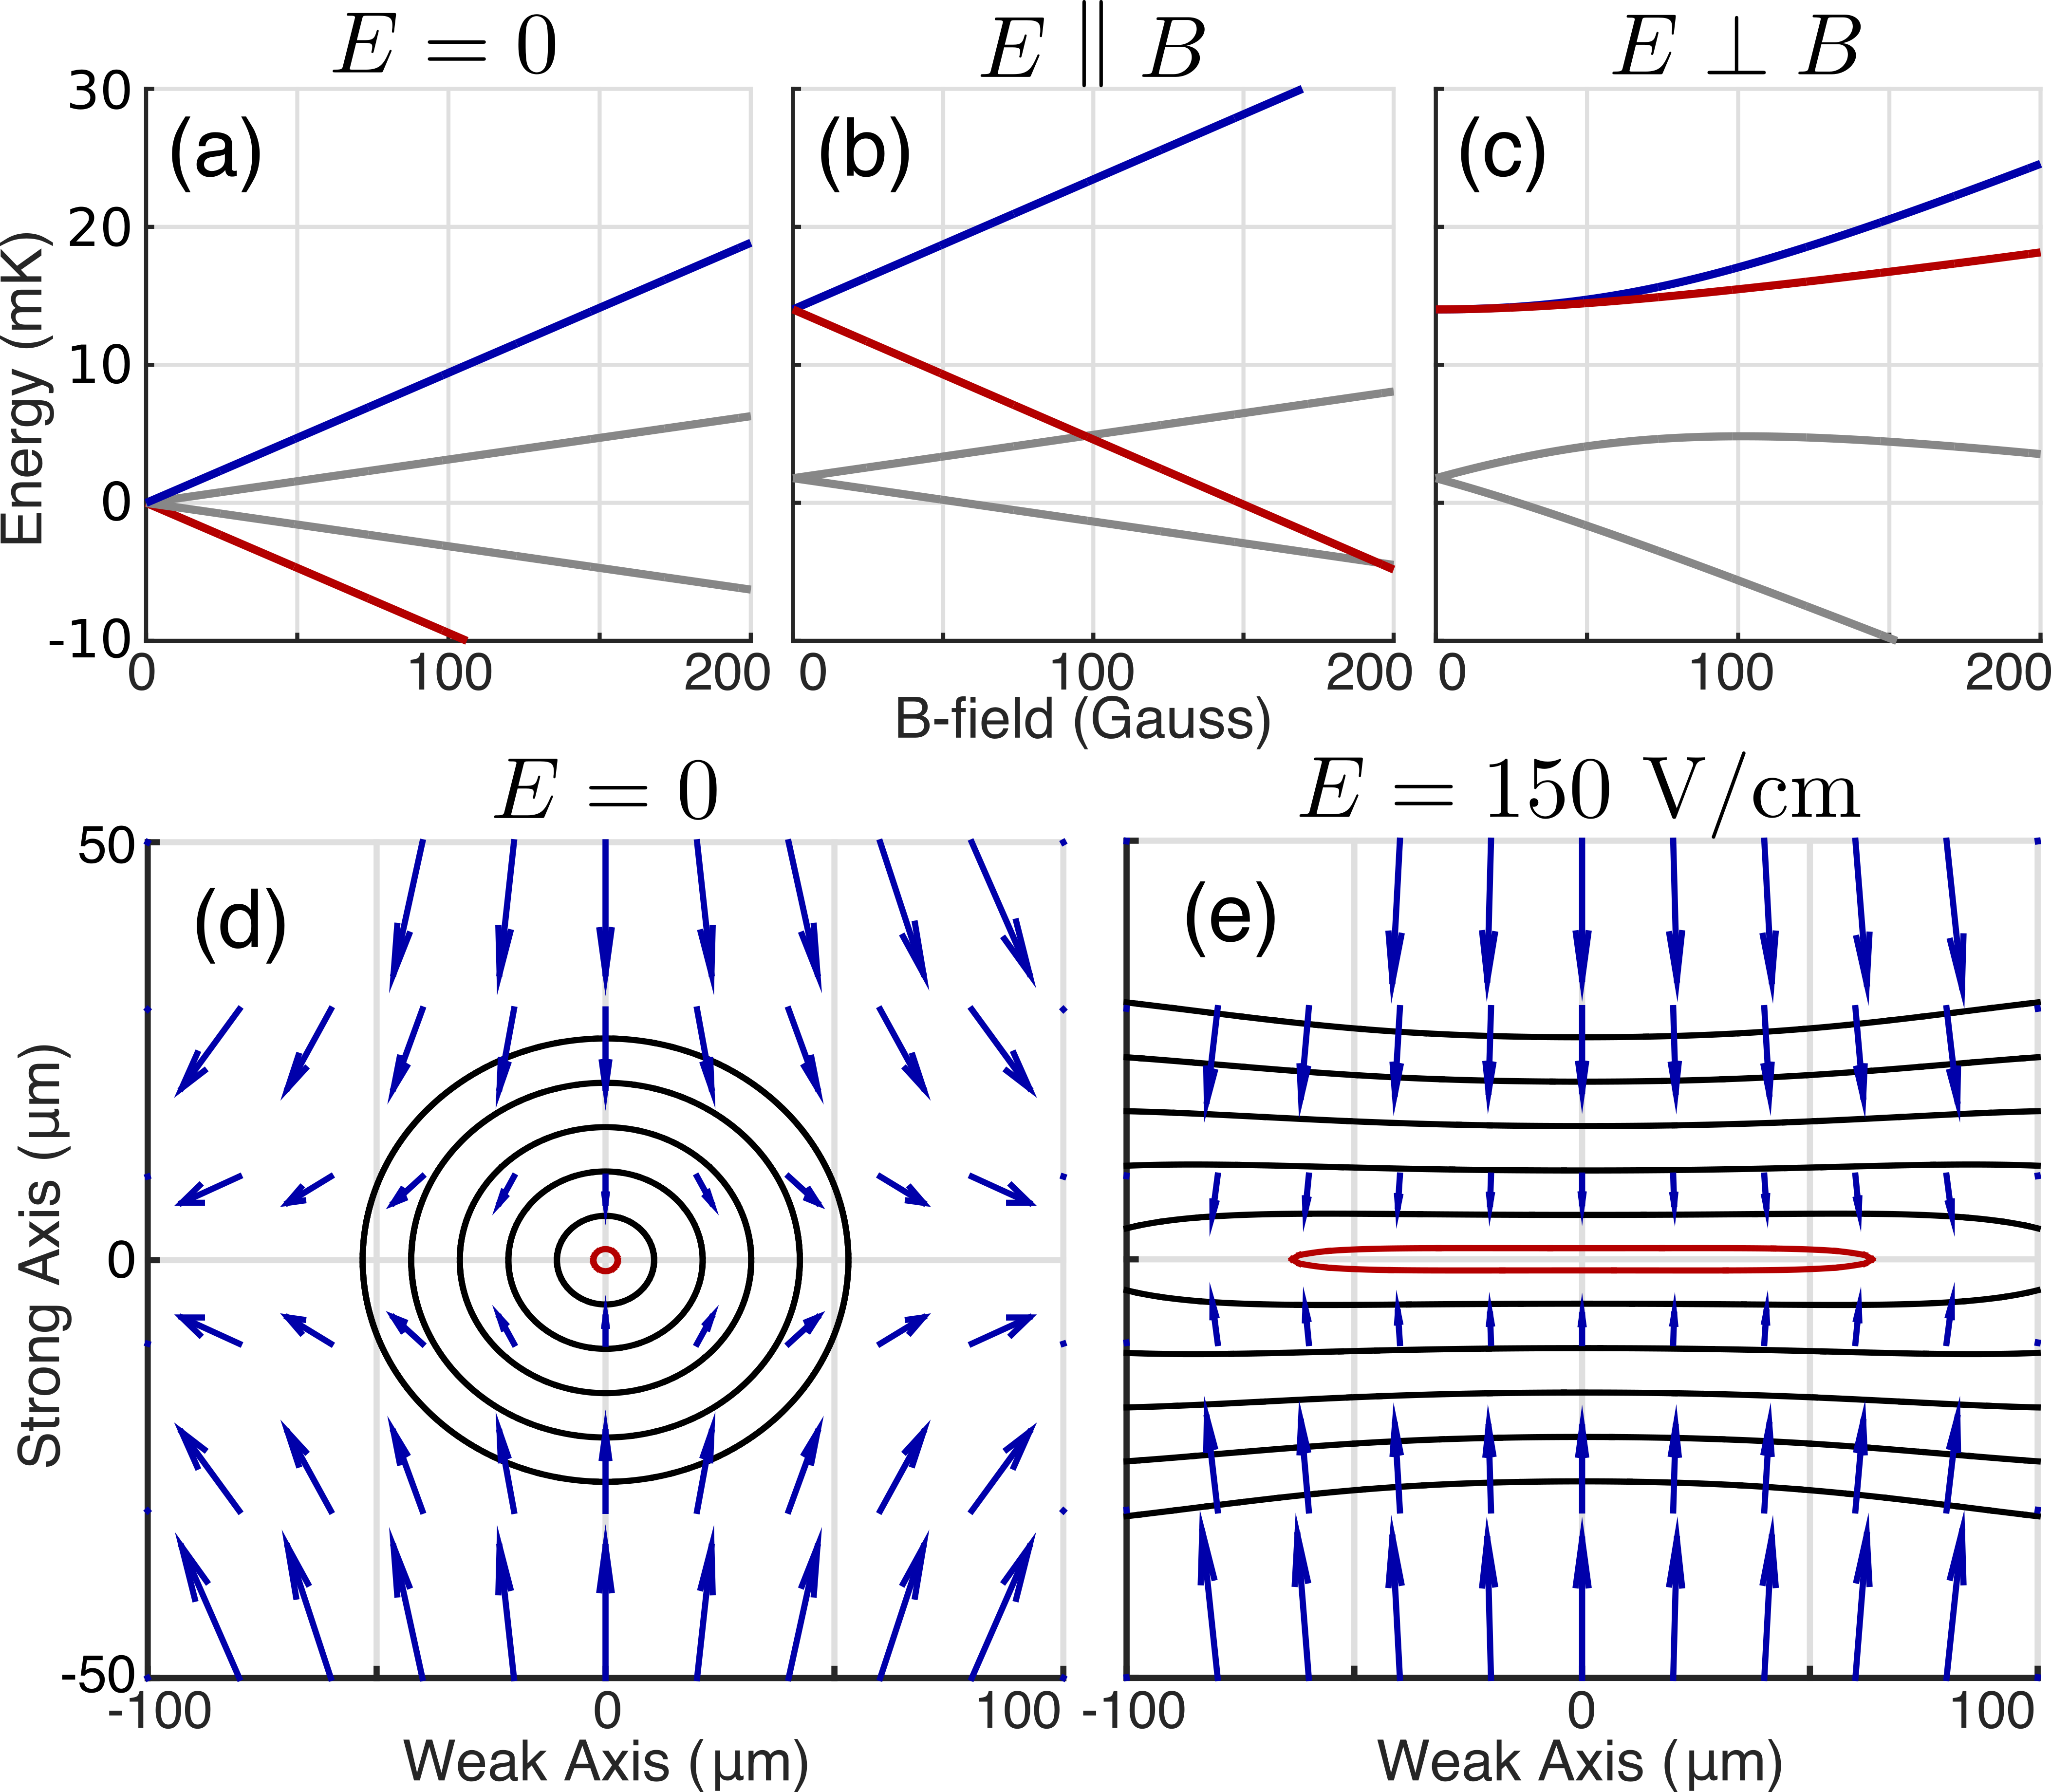
\includegraphics[width=86mm]{Blocking/blocking.png}%
\caption{
The blocking effect. (a), four Zeeman split lines in the ground state of OH. A nearly identical set of four states of opposite parity lie 100 mK below. The trapped state and it's spin flip partner are in blue and red. (b) Zeeman splitting with the addition of an electric field of 150 V/cm parallel to the magnetic field. (c) Again but with the fields orthogonal. The red state, untrapped in parallel fields, here draws very close to the trapped state in blue. A surface showing the behavior at all angles can be found in \cite{Stuhl2013}. (d) Contours of energy separation every 2 mK between the trapped and spin-flipped state near the zero of a 2 T/cm magnetic quadrupole trap without electric field. Magnetic field arrows in blue. (e) Again with 150 V/cm. Note the drastic widening of the lowest contour, in red. Here the vectors point along the direction of the local Hund's Case X quantization axis \cite{Bohn2013} and their magnitude gives the local potential energy of the trapped state relative to the trap center.
\label{fig:blocking}}
\end{figure}

To develop some intuition for this, we work in the basis of total angular momentum $J$ and parity $\epsilon$ which is appropriate for Hund's case (a). The eight states in this basis for OH's $J=3/2$ ground state are indicated by the state ket $|\epsilon\!=\!f,e\;;\;m_J\!=\!\pm1/2,\pm3/2\rangle$. An electric field splits states according to the absolute value of their $m_J$ number, with $|f,\pm3/2\rangle$ shifting upward strongly, $|f,\pm1/2\rangle$ one third as strongly, and the negative parity $|e\rangle$ states shifting oppositely. A magnetic field linearly splits states in proportion with $m_J$. Since we use electric fields for slowing and magnetic for trapping, only $|f,3/2\rangle$ are trapped. When an electric field has already set the quantization axis with respect to which $m_J$ is defined, the orthogonal magnetic field sees this as a coupling of $|f,3/2\rangle$ to $|f,-3/2\rangle$ which must be overcome. This is a $3/2-(-3/2)=3^\text{rd}$ order task, hence the cubic Zeeman splitting. If $E\parallel B$, this basis change is unnecessary and the Zeeman splitting is not blocked. For the $|m_J|=1/2$ states, realigning the quantization axis when $E\!\perp\! B$ is a $1/2-(-1/2)=1^\text{st}$ order task, so the splitting remains linear; see the gray lines close to zero field in panel (c) of fig.~\ref{fig:blocking}. Similarly, in ref.~\cite{Lara2008}, it was specifically undertaken to investigate the spin-flip loss for OH molecules in a magnetic quadrupole trap with superposed electric field, and no enhancement was found because a simplified $J=1/2$ Hamiltonian was used.

We can apply Brillouin-Wigner perturbation theory or analytically solve the ground state eigenenergies and taylor expand to obtain the following functional form for the Zeeman splitting between the $|f,\pm3/2\rangle$ states where $E\!\perp\! B$:

\begin{equation}
\label{eq:HZprop}
H_Z\approx \frac{(1.4\mu_BB)^3}{(1.7d_EE)^4}\Delta^2 f(\Delta,d_EE)
\end{equation}

\noindent Here $\mu_B$ and $d_E$ are the bohr magneton and the Debye, $B$ and $E$ are the corresponding field magnitudes, $\Delta$ is the lambda doublet splitting in energy units, and $f$ represents a complicated term of order unity for $d_EE < \Delta$ and order $d_EE/\Delta$ for larger $E$. We can use this to develop a scaling law for the enhancement. Let $\kappa$ be the energy threshold for gaps between states below which spin-flips are possible at the 50\% level. $\kappa$ depends on the mean velocity of trapped species and on the trap gradient near the hopping region, and so must be separately computed for any given scenario. For OH molecules in a  quadrupole trap \cite{sawyer2008} with strong gradient $2 \text{T/cm}$ and temperature $50 \text{mK}$, $\kappa=5\text{MHz}$. Without electric field, the effective cross sectional area for a hopping region is approximately $\pi (\kappa/\mu_BB\prime)^2$, approximating the ellipsoidal region given by $\mu_BB<\kappa$ as a flat disk. With electric field, a much larger magnetic field is required to overcome blocking, so we have from eq.~\ref{eq:HZprop} that $\mu_BB < \sqrt[3]{\frac{\kappa (d_EE)^4}{\Delta^2}}$, so for $d_EE>\sqrt{\kappa\Delta}$ there is an enhancement given by the following equation:
\begin{equation}
\nu = \left(\frac{d_EE}{\sqrt{\kappa\Delta}}\right)^\frac{8}{3}
\label{eq:blimit}
\end{equation} 

We can numerically evaluate the loss rates and enhancements for a thermal molecule distribution by performing an integral to calculate flux through the relevant loss plane weighted by the hopping probability on that plane. This is described more fully in the appendix, and is a significant improvement over previous attempts to evaluate this loss. The following table provides the results of these calculations for various conditions of experimental interest for OH molecules.

\newcommand{\shiftright}[2]{\makebox[#1][r]{\makebox[0pt][l]{#2}}}

\begin{table}[h]
\caption{Enhancements and loss rates for OH}
\label{tab:rates}
\begin{tabular}{c|cc|cc|c}
\hline\hline
 & \raisebox{-1.3ex}{\shiftright{4pt}{45 mK}} & & \raisebox{-1.3ex}{\shiftright{4pt}{5 mK}} & & \\
\raisebox{1.5ex}{$E$ field} & $\nu$ & $\Gamma\,(s^{-1})$ & $\nu$ & $\Gamma\,(s^{-1})$ & \raisebox{1.5ex}{Purpose} \\
\hline
0 V/cm 	& 1 		& 0.02 	& 1 		& 1.3 	& No Field \\
300 V/cm 	& 5 		& 0.1 	& 9 		& 11 		& Evaporation \\
550 V/cm 	& 17 		& 0.3 	& 40 		& 50 		& Spectroscopy \\
3 kV/cm 	& 1000 	& 19 		& 1600 	& 2000 	& Polarizing \\
\hline
\end{tabular}
\end{table}

%%%%%%%%%%%%%%%%%%%%%%%%%%
%  PIN TRAP GEOMETRY
%%%%%%%%%%%%%%%%%%%%%%%%%%


One obvious way to avoid the loss enhancement is to simply never use electric field in a magnetic trap. This prevents loss from being enhanced compared with atoms, but doesn't remove it entirely. Another possibility is to trap with electric fields, where no spin-flip loss is possible thanks to the $\Delta=h\,\cdot\,1.67\text{ GHz}$ splitting between the weak and strong field seeking states. However this splitting also results in a significant reduction in trap gradient close to the center, very undesirable for further cooling by evaporation. Moreover, there are reductions in inelastic to benefit from in magnetic fields. \cite{stuhl2012evap}

\begin{figure}
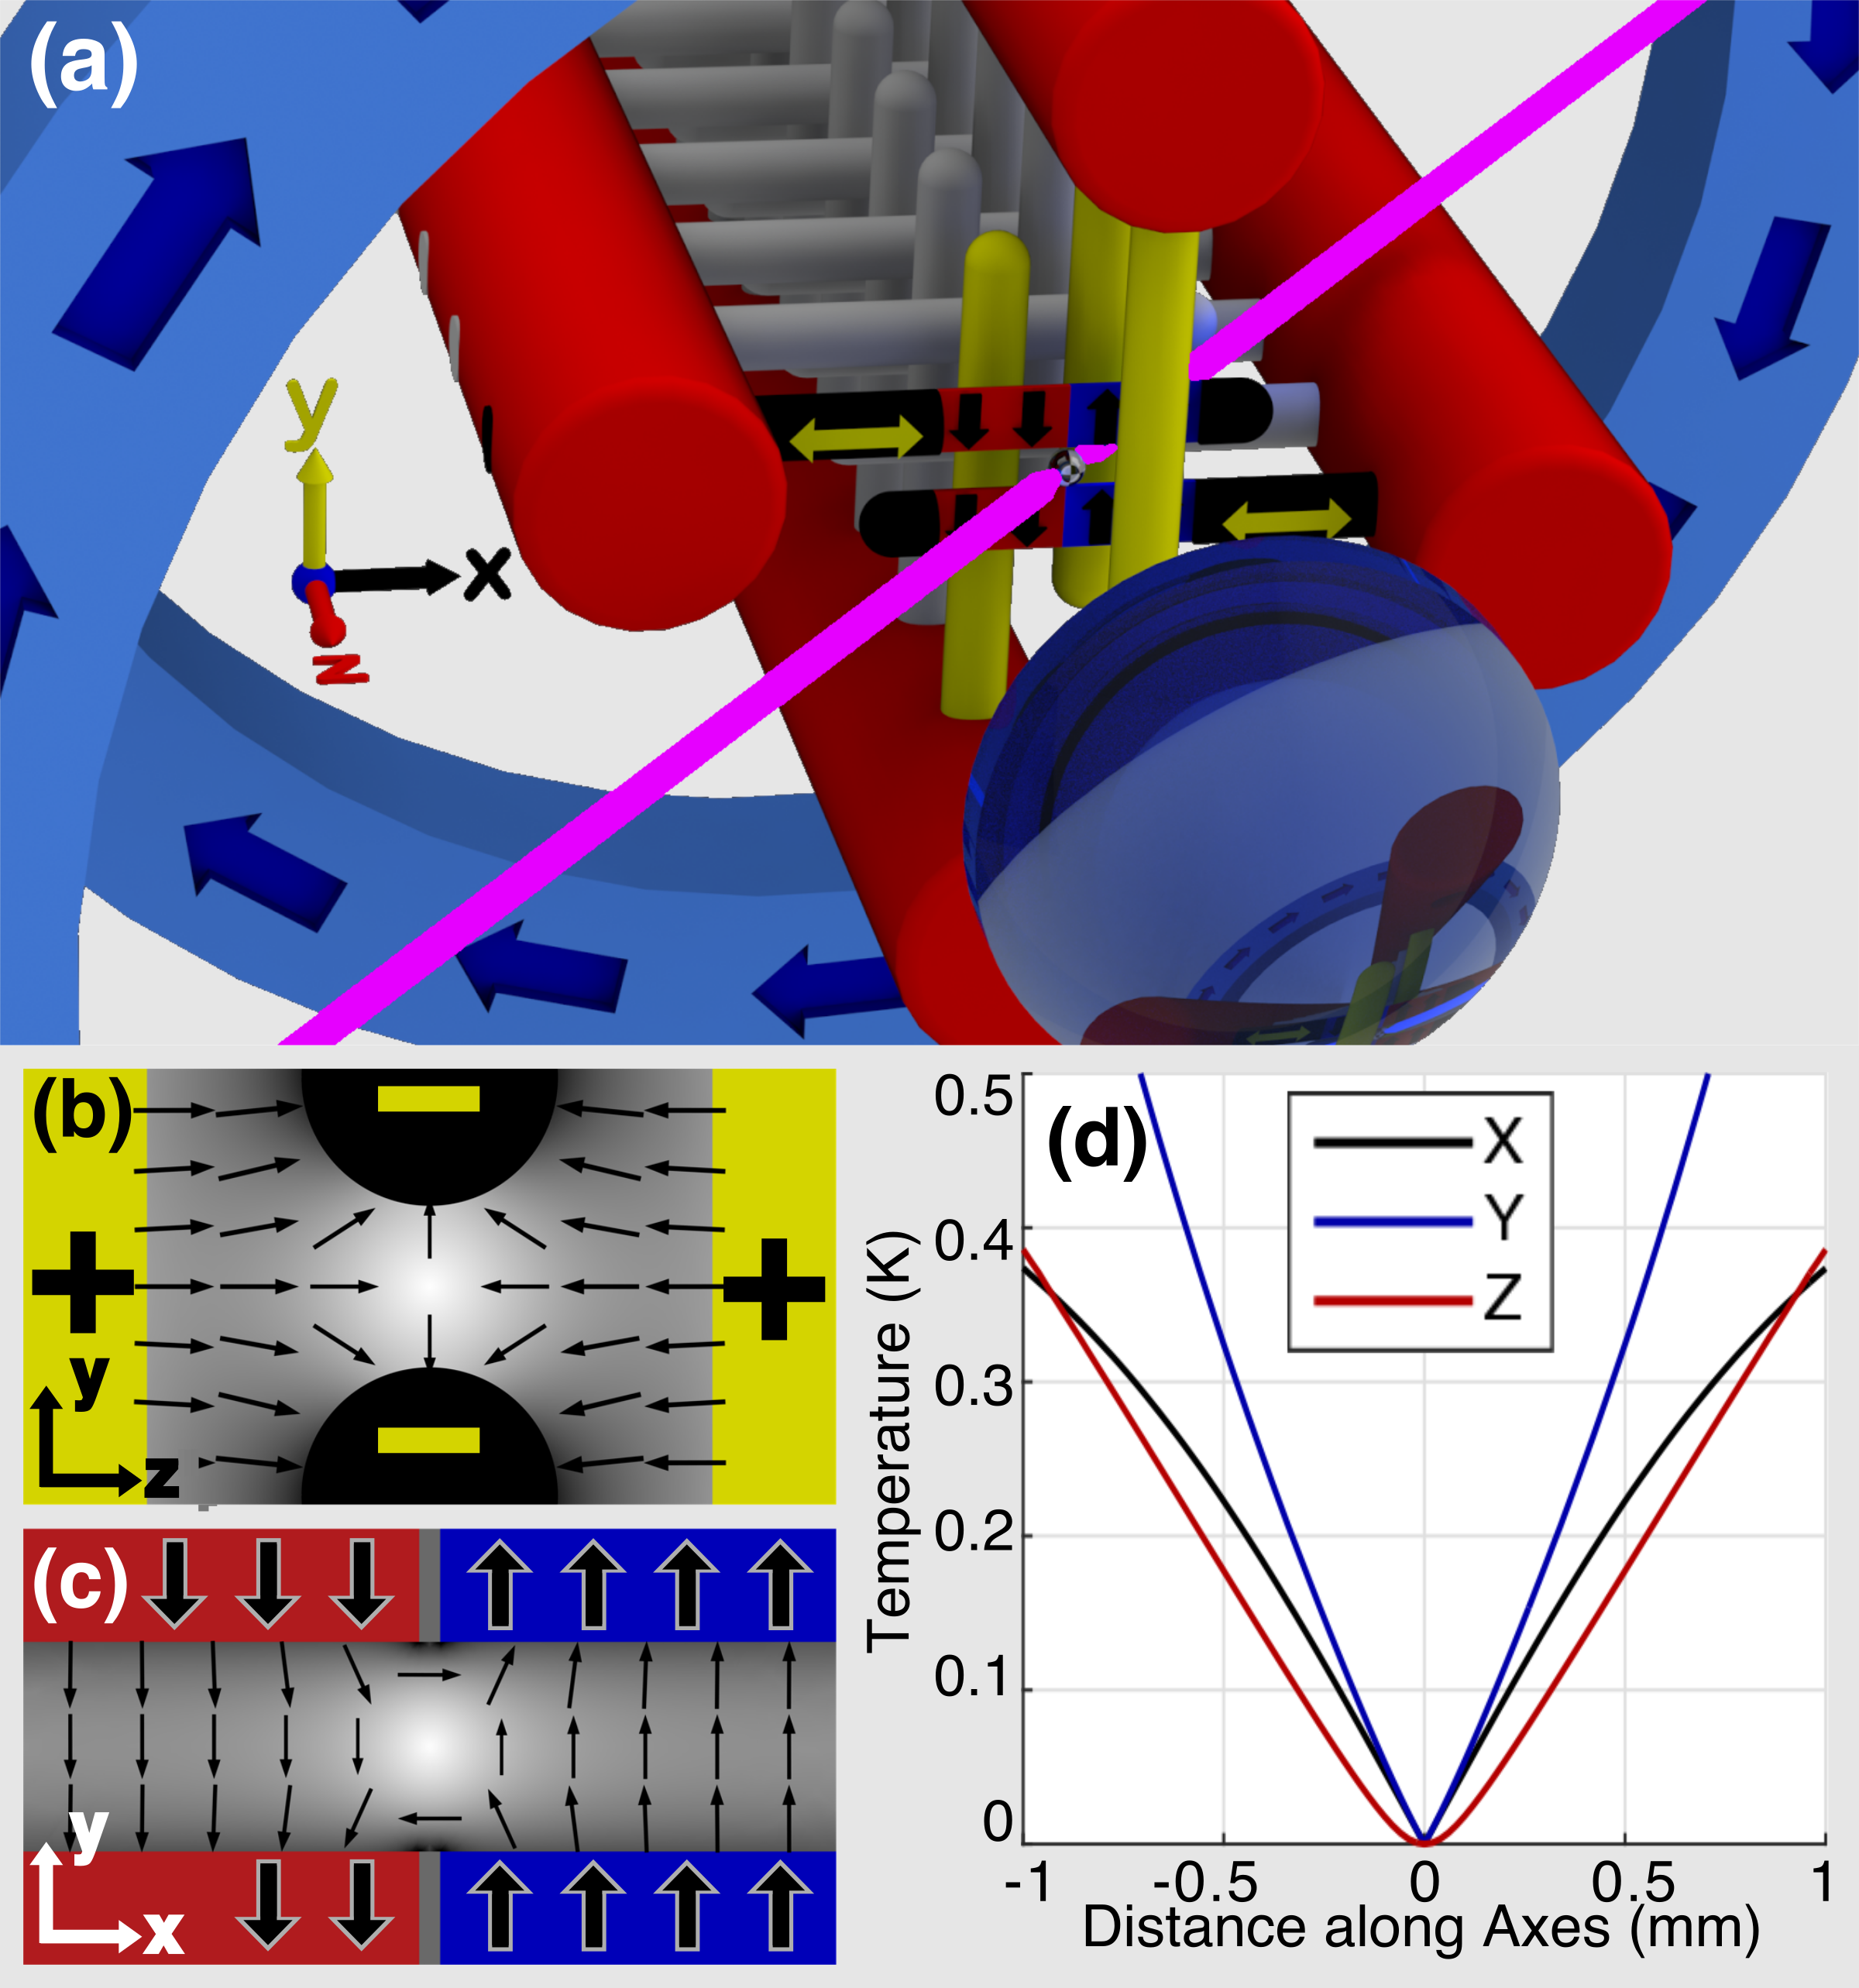
\includegraphics[width=86mm]{Geometry/CAD_recolor_laser_panels.PNG}%blue-red-yellow-v2_CAD.png}%
\caption{
Trapping is achieved by combining a radial magnetic quadrupole field, created by the magnetized second to last electrode pair of the decelerator, with a longitudinal electric quadrupole field created by the third to last and last electrode pairs, respectively (yellow, one electrode is omitted for clarity). The magnetized electrodes can be translated in situ along the x-axis to align their domains and optimize the quadrupole. As there is no trapping magnetic field in the z-direction in this configuration, macroscopic external bias coils can be used to lift the gap between the top two states of the OH ground-state manifold and thus tune the molecular loss. Detection is realized using laser induced fluorescence along the x+y-z direction (blue), which is collected using a lens system and PMT in the z-direction.
\label{fig:CAD}}
\end{figure}

Seeking to remove the loss entirely but without trap gradient sacrifice, we switch from a 3D to a 2D magnetic trap, and use an intersecting electric 2D quadrupole to plug the remaining direction (and incidentally add strength to one of the already trapped directions). This does not prevent $E\!\perp\! B$, but it allows us to tune the minimum $B$ field with an external bias coil oriented along the axis of the 2D quadrupole trap. This is similar to the Ioffe-Pritchard strategy \cite{pritchard1983}, where a 2D quadrupole is combined with an axial dipole trap. Typically, the axial and radial trapping interfere somewhat, resulting in significantly lower trap depths compared to the 3D quadrupole. We thwart this interference by the use of different fields for the axial and radial directions, which can ``block" one another as discussed earlier but never result in an absolute decrease in potential energy of the doubly weak field seeking substate. 

Serendipitously, we are able to achieve these fields with a geometry that exactly matches that of our Stark decelerator \cite{Bochinski2003}, as shown in fig.~\ref{fig:CAD}. OH molecules are created using a supersonic expansion source and decelerated from an initial velocity of 460m/s to a final velocity of 40ms/s using a Stark decelerator. The decelerator contains 142 electrode pairs. By magnetizing a pair of such pins in a dual domain manner, a 2D quadrupole is formed. The electric trapping in the third direction as achieved by charging the pin pair previous and following the magnetic pins to the same voltage, requiring only that high voltage switches be cascaded since normally pin pairs are oppositely charged. By intuition and by our phase space coupling simulations, this represents a near best-case scenario for coupling between a pulsed decelerator and a trap, although in practice we do not realize any significant molecule number increase relative to our previous geometries. This could be related to the difficulty of conditioning the magnet surfaces. For N38 magnets chosen so as to maintain magnetization during violent conditioning procedures, $B^\prime=5\text{ T/cm}$ and $E^\prime=100 \text{ kV/cm}^2$. These correspond to trap frequencies $\nu_x=3\text{ kHz}$, $\nu_y=5\text{ kHz}$, and $\nu_z=4\text{ kHz}$ for molecules traveling on the axes.

\begin{figure}
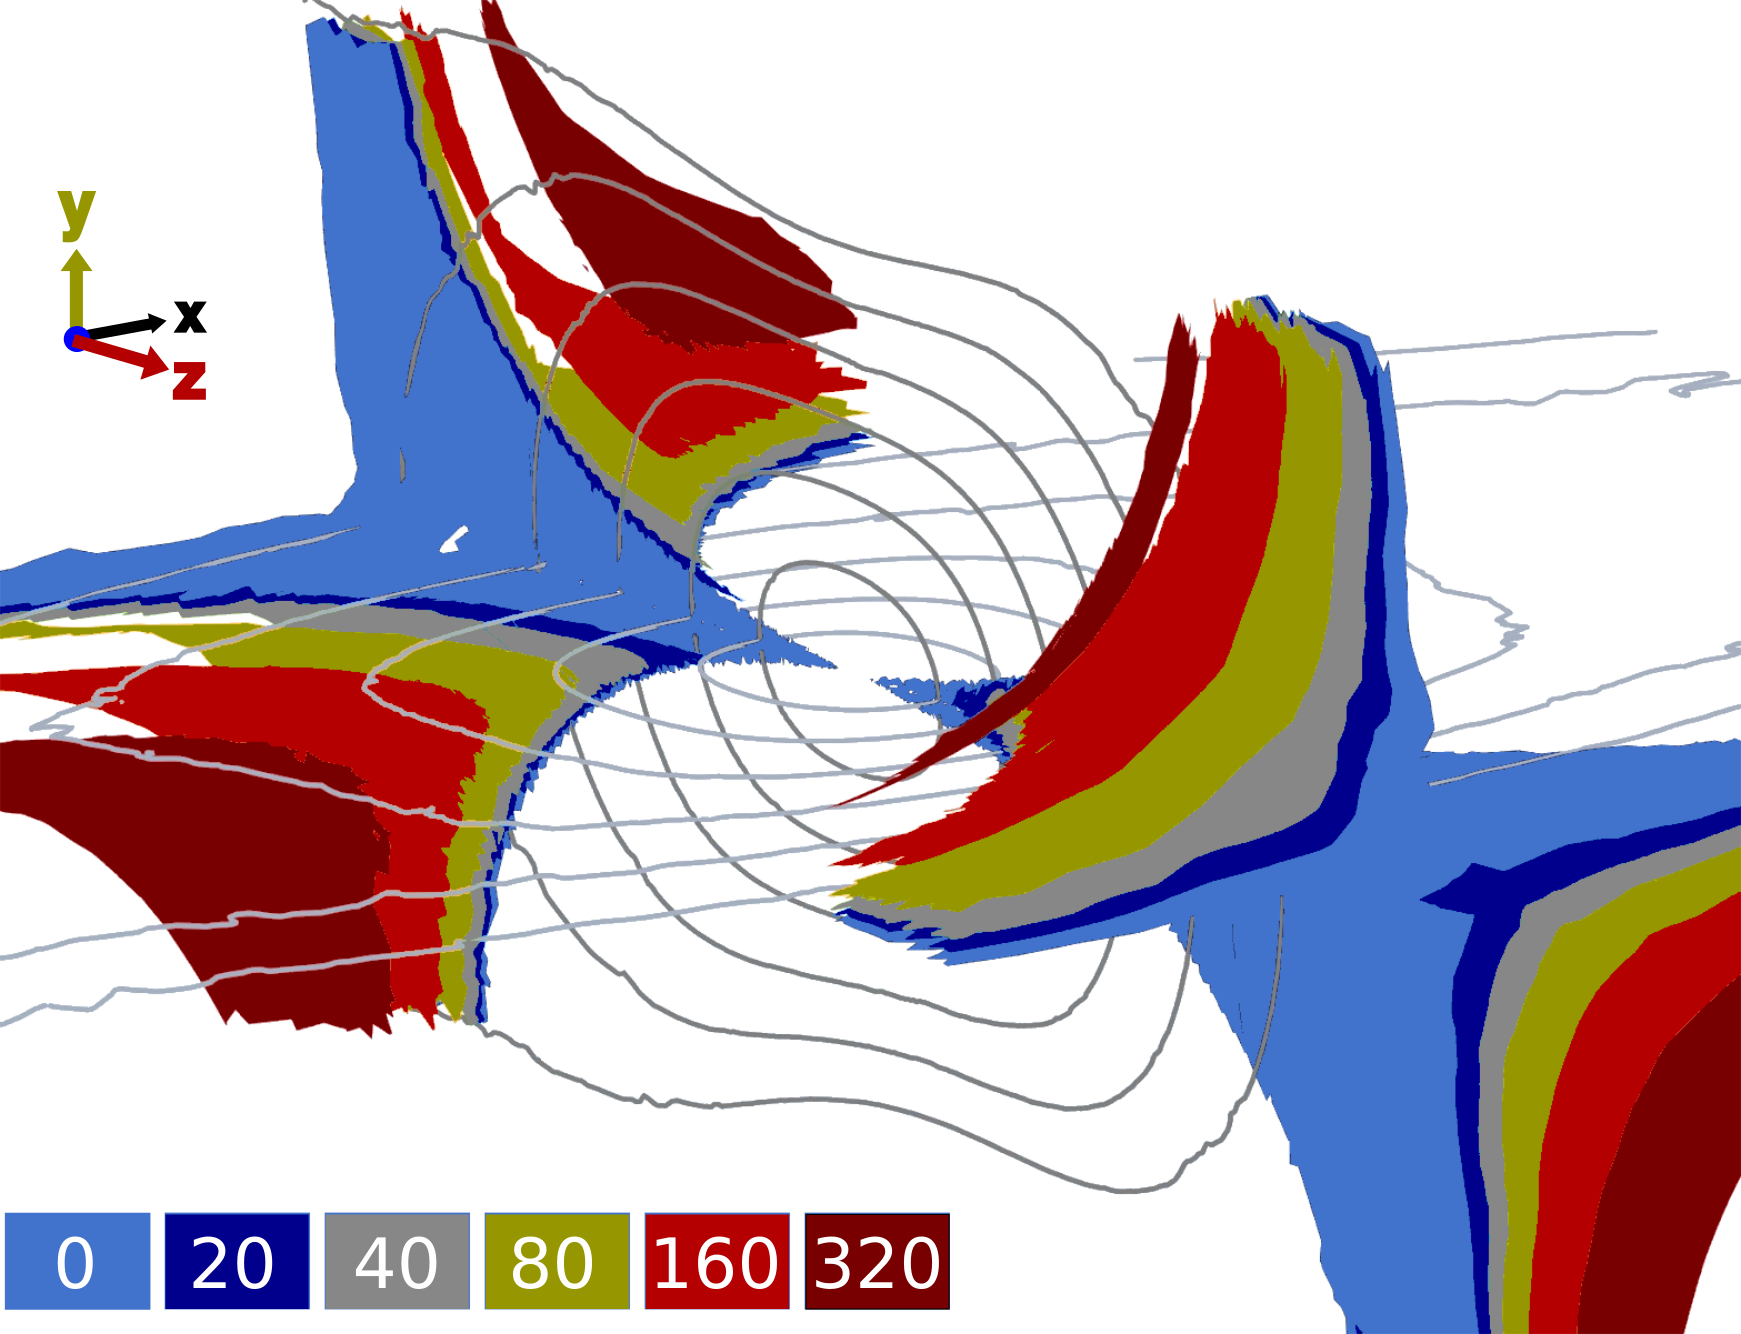
\includegraphics[width=86mm]{LossSurfaces/Loss_Surface_Chunks_recolored_legend.png}%
\caption{
Each color shows the surfaces where spin-flip can occur for the particular value of $B_\text{coil}$ given by the legend in units of Gauss. Trap energy contours are shown in gray. Larger $B_\text{coil}$ pushes the loss regions away from the trap center.
\label{fig:LSurfs}}
\end{figure}

Now regarding the molecule enhanced spin-flip loss, $E\!\perp\! B$ on a hyperbolic sheet which deviates more significantly from the z axis with increasing $B_{coil}$, and reduces to the pair of planes $x=0$ and $y=0$ in the limit that $B_{coil} = 0$. On this hyperbolic sheet, $B$ must be larger than the threshold set by Eq.~\ref{eq:blimit} to overcome blocking. Fortunately, $B_{coil}$ does not have to overcome the blocking limit, it only needs to push the $B\!\perp\! E$ surface slightly off the $z$-axis for the strong  quadrupole fields to overcome the blocking. In fig.~\ref{fig:LSurfs}, the surfaces where $B\!\perp\! E$ are colored wherever the splitting there is below the threshold $\kappa$. Note how $B_\text{coil}$ tunes the proximity of the loss regions to zero. The loss regions are never fully removed, but they can be tuned high enough that molecules accessing them could already escape the trap mechanically.

\begin{figure}
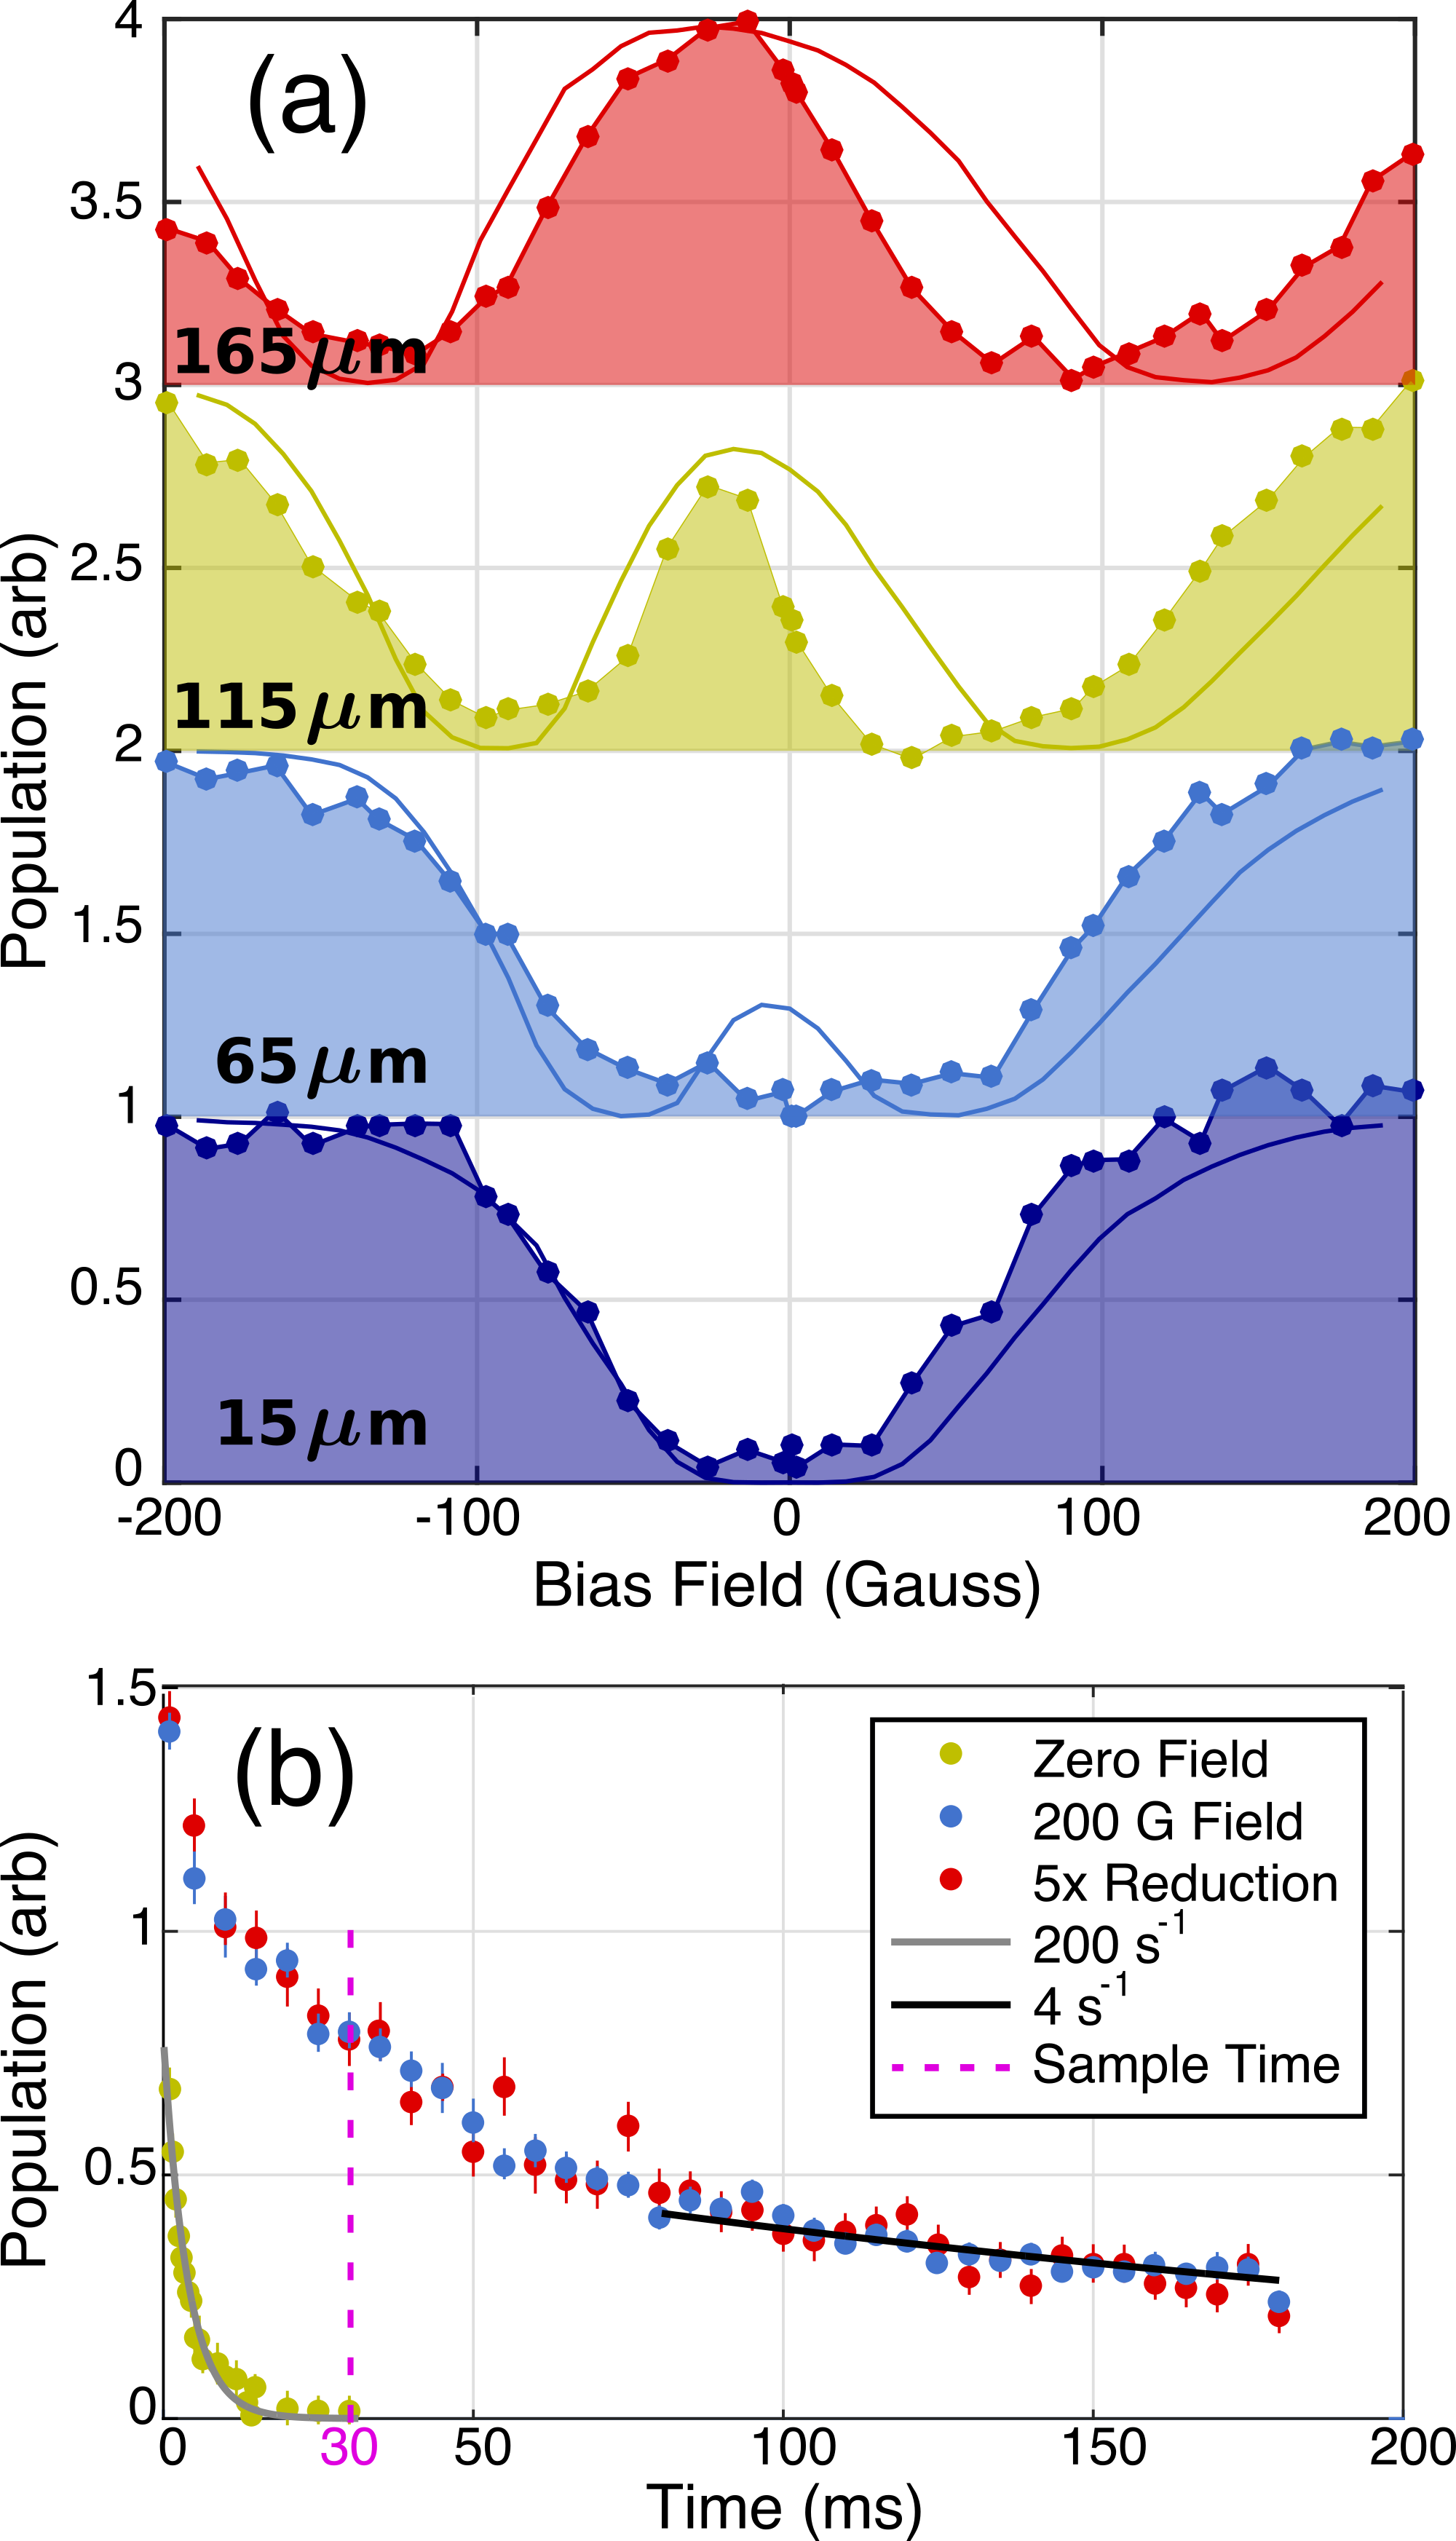
\includegraphics[width=86mm]{VWFig/tim-style-by-dave.png}%
\caption{
Family of curves showing the remaining population after $30 \text{ms}$ as a function of pin offset and magnetic bias field.
\label{fig:WVplot}}
\end{figure}

Unfortunately, the preceding picture only applies for well-aligned magnetic pins. Translations of our magnetic pins in their mounts lead to important modifications to the axial behavior of the magnetic trap that influence the tunability of the loss. Essentially, when the pairs of magnetic domains of the two pins are out of mutual alignment by a distance $d$, a small trapping field $\vec{B}\propto B^\prime z\hat{z} d$ is introduced along the otherwise magnetic-field-free z-axis. This means that $B_\text{coil}$ no longer directly tunes the minimum magnetic field in the trap. Instead, $B_\text{coil}$ must first overcome the slight trapping field along the $z$-axis, translating a point of zero field along the z axis and eventually out of the trap. In order to really disentangle this effect from our results, we installed an in-situ pin translation stage and obtained the family of curves shown in fig.~\ref{fig:WVplot}. With the pins tuned into alignment, $B_\text{coil}$ of either sign suppresses the loss in agreement with fig.~\ref{fig:LSurfs}. Otherwise, $B_\text{coil}$ first increases the loss by moving the magnetic zero into regions of large electric field, but eventually overwhelms it, producing a characteristic double-well shape. 

As a quantitative companion to this intuition for the double-well structure, we fit the family of curves shown in fig.~\ref{fig:WVplot} by performing a detailed numerical integration of spin-flip loss flux over all hyperbolic planes where loss can occur, weighted by the expected Maxwell-Boltzmann distribution of molecules in the trap. The computation is performed in COMSOL Multiphysics, with cloud temperature as the only free parameter. Source-code for the model is available.\cite{githubCOMcode} The fit temperature is approximately $100\pm10\text{ mK}$. This temperature is twice that of our previous traps, most likely due to the increased trap depth but potentially related to conditioning challenges for the magnetic pins.

\begin{figure}
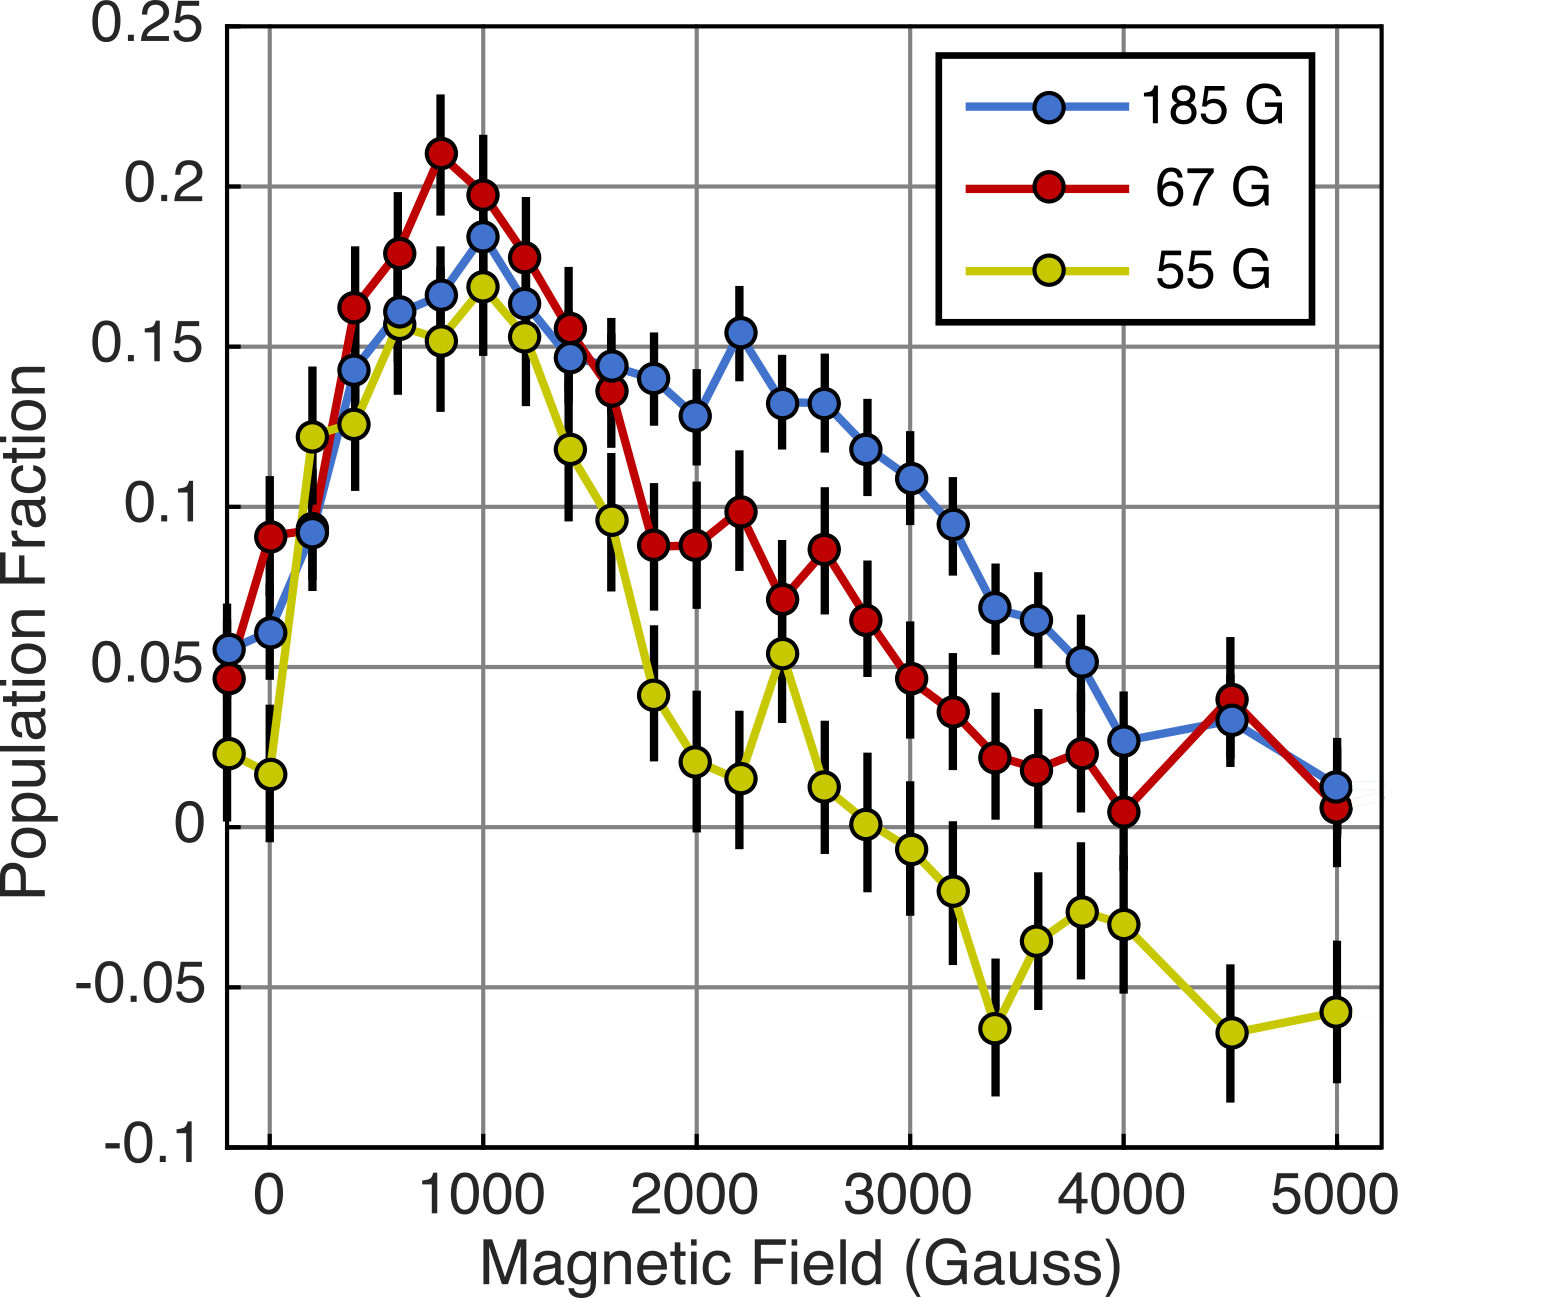
\includegraphics[width=90mm]{MWSpec/MW-therm-dave.png}%
\caption{
Microwave Thermometry in the trap.
\label{fig:spec}}
\end{figure}

To further validate the claim that $B_\text{coil}$ tunes loss away from the trap center, we perform a Zeeman microwave spectroscopy along the $|f,3/2\rangle$ to $|e,3/2\rangle$ line as in our previous work \cite{stuhl2012evap}. Rather than using a bias tee setup, a dangerous prospect with our trap deeply integrated in the high voltage decelerator, we use a home-made microwave probe to directly excite free space cavity modes of our vacuum chamber. The results are shown in fig.~\ref{fig:spec}. With the magnetic pins aligned, it is seen that higher values of $B_{\text{coil}}$ indeed increases the population of molecules able to survive at higher fields. In order to perform this spectroscopy, the trapping electric fields are switched off immediately prior to the application of a microwave transfer pulse tuned to a particular magnetic field strength. Thus the results reflect the Zeeman potential energy only. Roughly speaking, the average field of $2\text{ kG}$ corresponds to $200\text{ mK}$ for OH. Since this is approximately half the potential energy, we have $U\approx400\text{ mK}$. From the virial theorem for a linear trap, $U = 4.5k_BT$, so we can say the spectrum is consistent with $T\approx 90\text{ mK}$ and consistent with our fitting in fig.~\ref{fig:WVplot}.

In the case of lowest applied magnetic field in fig.~\ref{fig:spec}, i.e. deepest cutting of the loss region toward the trap center, a negative going signal is observed. This indicates a build-up in the opposite parity $|e,3/2\rangle$ state. Although the spin-flips we have discussed connect $|f,\pm3/2\rangle$, the $|f,-3/2\rangle$ state actually remains trapped thanks to adiabatic transitions to $|f,1/2\rangle$ and later $e,3/2\rangle$ facilitated by the large $E$ fields present in the trap. This secondary state is much more weakly trapped and exhibits molecule enhanced spin-flip loss to other lower states, although the enhancement is related to a quadratic blocking of the zeeman splitting near the intersection of $|f,-3/2\rangle$ and $|f,1/2\rangle$, and is thus not as dominating as the loss in the primary state due to cubic blocking.

Once the loss is fully removed, we observe the trend shown in fig.~\ref{fig:timetrace}. The decay rate decreases with population over a timescale that is long compared with trap frequency and is thus suggestive of a collisional process. However, we implement a completely phase-space blind density reduction technique to significantly reduce our molecule number and observe little change in the shape of the trend, indicating that primarily single-particle physics is responsible. We suspect that the trend is related to the persistence of high energy chaotic orbits which can possess long escape times, as seen in other exotically shaped trapping potentials \cite{Gonzalez-Ferez2014}. We hope in the near future to implement an increase in molecule number rather than a decrease, by means of a suite of density enhancing experimental improvements slated to come online.

We have conclusively demonstrated the existence of molecule enhanced spin-flip loss by tuning it from an overwhelming rate to complete removal. Our explanation of the loss provides detailed predictions of how its position and magnitude ought to scale with bias field and trap alignment, which we have experimentally verified. Our results contradict existing predictions about molecule enhanced spin-flip loss and we provide a consistent framework that explains this. Beyond merely demonstrating the loss, we have devised a viable trapping geometry in which it is fully mitigated without trap-depth sacrifice, paving the way toward further improvements in molecule trapping and cooling.

%\appendix
\begin{eqnarray}
\vec{B} &=&  B^\prime y\hat{x}+ B^\prime x\hat{y} + B_{coil} \hat{z}\\
\vec{E} &=&  E^\prime y\hat{y}-  E^\prime z\hat{z}
\end{eqnarray}

\begin{eqnarray}
\vec{B}\cdot \vec{E} &= 0\\
B^\prime x E^\prime y - B_{coil}  E^\prime z &= 0\\
B_{coil}z &= xyB^\prime
\end{eqnarray}

\begin{equation}
\gamma_\text{flip}=\frac{\int\limits^\infty_0 2\pi r e^{-r/r_0} \int\limits^\infty_{-\infty} e^{-mv_z^2/kT} |v_z| e^{-2\pi\Gamma(r,v_z)}dv_zdr}{\int\limits^\infty_0 2\pi r e^{-r/r_0} \int\limits^\infty_{-\infty} e^{-mv_z^2/kT} dv_zdr}
\end{equation}

%includes uncited bib entries
\nocite{*}
\bibliographystyle{apsrev4-1_no_Arxiv}
\bibliography{MolecularMajoranaLoss}% Produces the bibliography via BibTeX.

\end{document}
%
% ****** End of file MolecularMajoranaLoss.tex ******
